
\section{Solving P1: Pair Within Distance}
\label{solving_P1}

Checking whether two given strings are within a certain \gls{error distance} is a well-known problem. In the case of \gls{Hamming distance}, it is simply the count of \glspl{mismatch} between symbols compared pairwise between the given strings for all the string indices.
 
In the case of \gls{edit distance}, much extensive work exists. Edit distance (here shortened to `ed') between strings $X$ with length $x$ and $Y$ with length $y$ can be defined recursively:
% //
% \vspace{1mm}
\[ 
\text{    ed(X,Y)} = min\left \{
\bgroup
\def\arraystretch{2}
\begin{tabular}{p{6.2cm}|p{3cm}}

ed($X[1,x]$, $Y[1,y-1]$) + 1
&\gls{insertion} case
\\
% \hline
ed($X[1,x-1]$, $Y[1,y]$) + 1
&\gls{deletion} case
\\
% \hline
ed($X[1,x-1]$, $Y[1,y-1]$) + z
\newline{}
where $z=1$ if $X[x]\neq{}Y[y]$ else 1.
&\gls{substitution} or match case
% \\

\end{tabular}
\egroup
\right \}
\]
% \vspace{2mm}

A well-known dynamic programming solution builds a table incrementally, with each cell storing the edit distance between unique pairs of prefixes of the input strings. Further optimizations exist to avoid populating the entire table, but they are beyond the scope of this work.








\section{Solving P2: Approximate String Match}
\label{solvingP2}


P2 is the problem explored by \kark{} in~\cite{kark2007}. More difficult than P1, P2 can be naively decomposed into numerous instances of P1 subproblems. However, this is not the only approach possible. By using a \gls{text index}, a much smarter algorithm can find the same \glspl{solution} in less time by leveraging the shared work done for different possible \glspl{derived string} of the same string. However, as demonstrated by the \glspl{filter algorithm} to come, use of an index alone could still be considered naive.




\subsection{Solving P2 Using a Text Index} \label{P2text_index}

Finding all exact instances of a given string inside a \gls{text} is the job description of a \gls{text index}, designed to quickly locate occurrences of a given \gls{query} string within the prepared text. It is then only a matter of extending their functionality to find \glspl{approximate match} within the text by considering \glspl{derived string} producible from the query string by permitting \glspl{error}. A number of well-researched text indices exist which are suitable for this purpose. Our work uses a version of the \textit{FM-Index} with a simulated forward-search procedure. For more details on indices and the FM-Index in particular, see Section \ref{aux_info}. For more details on the simulated forwards search, see Section \ref{own_impl_search_dir}.
 
The FM-Index makes use of an iterative search procedure for exact occurrences of a given query\footnote{We find that considering the text index a black-box that interacts with the rest of the system in a call-response fashion a useful metaphor for understanding the nature of the search. As such, `query' refers to whatever full string the text index is searching for, with the set of match locations returned being the `response'.} string, iterating over symbols in the query one at a time while keeping track of \glspl{match location} inside the text every step of the way. Intuitively, this process begins with a set of match locations (initialized as the full range of the text), and gradually thins the set out. Throughout the search, match locations mark text substrings \textit{equivalent} to the prefix\footnote{Although this holds conceptually, in practice, this matching occurs in reverse (matching longer suffixes instead). This is discussed further in Section \ref{own_impl_search_dir}} of the query string matched so far. If no match locations remain, the search terminates. If the entire query string is matched, match locations are returned, representing occurrences of the query string within the text.
 
The idea behind the \gls{K-approximate} search is to generate all possible $K$-approximate derivations of the A string recursively. To achieve this, the search begins provided a new parameter \bfit{pE} (for `permitted errors'), initialized to $K$. As before, query symbols are considered one at a time, at each step narrowing down the set of match locations (and representing an incrementally-longer matched prefix of the query). However, instead of pruning matches that differ from the query string, when the \bfit{pE} parameter allows, the search retains match locations that \gls{mismatch} with the next query symbol, `spending' a permitted error (decrementing \bfit{pE}) for those match locations. As the search considers all match locations in batches, it needs to associate appropriate \bfit{pE} values for each match location; As shown in fig \ref{fig:index_search}, this is achieved by recursively branching the search for each symbol, partitioning the remaining match locations and pruning branches with empty match location sets.


\begin{figure}[!h]
\centering
\tikzset{
  treenode/.style = {align=center, inner sep=0pt, text centered,
    font=\sffamily},
  arn_n/.style = {treenode, circle, white, font=\sffamily\bfseries, draw=black,
    fill=black, text width=2.2em},% arbre rouge noir, noeud noir
  arn_r/.style = {treenode, circle, red, draw=red, 
    text width=2.2em, very thick},% arbre rouge noir, noeud rouge
  arn_x/.style = {treenode, rectangle, draw=black,
    minimum width=0.5em, minimum height=0.5em}% arbre rouge noir, nil
}

\begin{tikzpicture}[->,>=stealth',level/.style={sibling distance = 3cm/#1,
  level distance = 1.1cm, scale=1.2}] 
\node [arn_n] {$\epsilon$}
    child{ node [arn_n] {T} 
            child{ node [arn_n] {TT} 
            	child{ node [arn_n] {TTC} edge from parent node[above left]
                         {exact match}} %for a named pointer
							child{ node [arn_r] {TTT}}
            }
            child{ node [arn_r] {TC}
            		child{ node [arn_r] {TCC}}	
            }                            
    }
    child{ node [arn_r] {C} 
            child{ node [arn_r] {CT} 
              	 	child{ node [arn_r] {CTC}}
            }
		}
; 
\end{tikzpicture}
\caption[Search tree of 1-approximate matching.]{Search tree for 1-approximate matching of `TTC' using a text index with alphabet $\{T, C\}$. Black nodes have \bfit{pE}$=1$ and red nodes have \bfit{pE}$=0$.}
\label{fig:index_search}
\end{figure}

In practice, further unique branches are generated for each newly-matched symbol, as by the nature of the FM-Index, it is only possible to retain a subset of the match locations according to a \textit{specific symbol} at a time. 



Branches of the $K$-approximate search that reach the end of the query string represent \glspl{exact match} for strings \textit{derived} from the query (analogous to \textit{approximate} matches for the query). These leaf nodes each return return a set of match locations, the union of which represent the solution set of the problem.







\subsection{Solving P2 Using Substring Filters} \label{p2substring}

A \gls{substring filter} algorithm can be employed to reduce the search space of P2. The correctness of the \gls{filter criterion} is reliant on lemma \ref{lemma1}, originally provided by \kark{}, where it was called `Lemma 1.1'~\cite{kark2007} .

\begin{lemma}
\label{lemma1}
If a string containing no more than $K$ symbols $\phi{}$ is partitioned into $K+1$ blocks, at least one block must have $0$ $\phi{}$'s.
\end{lemma}

Term $\phi{}$ is any arbitrary symbol, but we consider the case when $\phi{}$ refers to an \gls{error} in the \gls{derivation} from some other string $X$. These errors occur at index positions and fall into partition \glspl{block} as any symbol would. Lemma \ref{lemma1} is based on something akin to the pigeonhole principle. As the \gls{string partition} also partitions the set of errors, the lemma observes that with more blocks than errors, there must be at least one block without any errors at all. 

To satisfy the precedent of the lemma, the substring algorithm begins by partitioning the given \gls{pattern} into $K+1$ blocks for a given \textit{error limit} argument $K$. A \gls{text index} is built for the \gls{text} as before. Now, instead of querying the index for all approximate instances of the entire $A$ string monolithically (as described in Section \ref{P2text_index}), the algorithm instead performs a \textit{set} of \glspl{query}. For each block of the pattern's partition, the index is queried for \glspl{match location} of just that single block in the text, allowing for no errors whatsoever. For each location of a complete block in the text found this way (with no errors all the way to the end), a \gls{candidate} is generated to mark a possible occurrence of an \gls{approximate match} of the pattern.

Each block’s query yields a set of candidates and the union of these sets is called the \textit{candidate set}. Observe that thanks to lemma \ref{lemma1}, as long as every pattern block is queried, any actual \gls{K-approximate} matches of the pattern string must bring rise to a candidate in one or more block's queries; The candidate set \textit{covers} the solution set. However, it does not hold that every candidate is a \gls{solution}; Candidates are generated to represent overlaps involving some substring occurrent at a match location in the text; However, the symbols of blocks \textit{adjacent} to this substring's blocks are not checked at all; They might be fraught with errors, or be predicted to extend beyond the bounds of the text. Finding the subset of candidates that are also solutions is done by iterating over candidates, retaining only candidates that satisfy the \gls{solution criterion}, `verifying' them to be solutions. This \gls{verification step} can be solved as an instance of P1.
 
The substring filter algorithm reduces cost by taking measures \textit{likely} to reduce the search space; Some cases don’t save time at all. Consider the following P3 problem:
\begin{align*}
\text{pattern}  &= \text{`GGGG'}\\
\text{text} &= \text{`GGGGGGGGGGG'}
\end{align*}

Approaching this instance with substring filters would produce a storm of candidates as very many \glspl{exact match} of pattern blocks will be found. In such a case, the filter provides no utility at all, and the algorithm degenerates to something akin to naively considering all possible derivations at all possible locations in the text. Thankfully, in practice, the majority of realistic problem instances have sparser solutions than the example above, and more effectively filter the search space.
 
Note the correctness of the algorithm is defined for arbitrary pattern partitions, so long as there are at least $K+1$ partition blocks. However, the manner in which the pattern is partitioned contributes significantly to computational cost. Consider the following instance with partitions already chosen:
\begin{align*}
\text{pattern:  } P &= `0000111101'\\
P_1 &= `0000' & P_2 &= `1111' & P_3 &= `01'\\
\text{text} &= `0101010101'
\end{align*}

Although this text certainly contains no matches of this pattern, it \textit{does} contain very many occurrences of the entirety of $P_3$, generating 5 \textit{spurious} candidates. Circumstances of this nature become more probable with short pattern blocks.







\subsection{Solving P2 Using Suffix Filters}
\label{P2suffix}

The \gls{suffix filter} algorithm described by \kark{} is quite similar to the \gls{substring filter} algorithm described in Section \ref{p2substring} above. The difference lies with its efforts to have a stricter \gls{filter criterion}, such that some more time is spent in the \gls{search step} generating a smaller set of \glspl{candidate}, and much less time is spent in the \gls{verification step}. The \gls{solution} set remains unchanged from the other P2 algorithms described so far.
 
The correctness of the suffix filter algorithm relies on lemma \ref{lemma2}, paraphrased from \kark{}'s paper, where it is called `Lemma 2.1'~\cite{kark2007}.


\begin{lemma}
\label{lemma2}
Consider only non-empty \glspl{block sequence}. If a string has a partition $Z$ with more blocks than symbols $\phi{}$, in at least one of $Z$'s \glspl{suffix block sequence} $S_Z$, for all \glspl{prefix block sequence} $P_{SZ}$ of $S_Z$, the number of blocks in $P_{SZ} >$ the number of $\phi{}$'s in $P_{SZ}$.
\end{lemma}

Lemma \ref{lemma2} can be understood as a natural consequence of Lemma \ref{lemma1}, applying under the same conditions but making a different observation. Assuming the premise holds, it guarantees for at least one suffix block sequence $S_Q$ of the pattern string, $Q$, the following is true:
When iterating over blocks in any prefix block sequence $P_{SQ}$ of $S_Q$ from left to right, there will always be strictly fewer cumulative errors encountered in $P_{SQ}$ than cumulative blocks counted.
 
To understand why lemma \ref{lemma2} holds, consider walking over all partition blocks of the string from left to right, counting encountered \glspl{error} at each block (inclusively). As there are fewer errors in total than blocks, at some stage during the iteration the cumulative number of errors must fall behind the index of the current block, never to catch up. It is at this moment that the suffix block sequence with the desired property begins. This `walking' description is rather suggestive of how the lemma is actually applied in the \gls{search step}.

As with the substring filter algorithm, the suffix filter algorithm begins by constructing a \gls{text index} for the given text string. The given pattern is again partitioned into $K+1$ blocks; However, where before \glspl{query} were performed for each pattern \textit{block}, the suffix filter algorithm performs a query for each \textit{suffix block sequence} of the pattern instead; The difference is outlined in Figure \ref{fig:substring_vs_suffix}.

\begin{figure}[!htb]
\centering
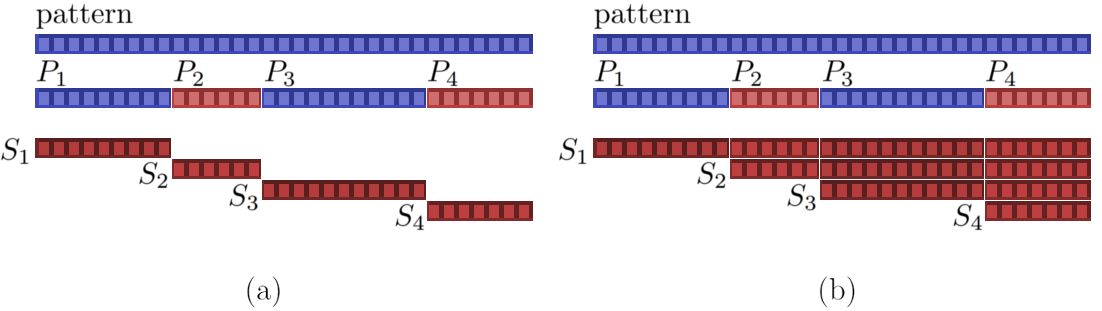
\includegraphics[width=1.0\textwidth]{images/substring_suffix.png}
\caption[Pattern string blocks vs. suffix block sequences for substring and suffix filter algorithms.]{Pattern string partitioned into blocks $[P_1, P_2, P_3, P_4]$, bringing rise to sequence of queries $[S_1, S_2, S_3, S_4]$. (a) Queries of the substring filter algorithm, one query per block of $P$. (b) Queries of the suffix filter algorithm, one query per suffix block sequence of $P$.}
\label{fig:substring_vs_suffix}
\end{figure}

As in the substring filter algorithm, the search process walks over query symbols one by one, keeping track of incrementally-longer \gls{match location} sets in the text throughout. Only now, the query string is comprised potentially of numerous blocks instead of just one. The search makes use of a parameter \bfit{pE} as it did in the indexed P2 algorithm, but this time it is initialized at $0$, effectively prohibiting any error-branching at first. Every time the search walk crosses over the end of a block, the search \textit{accumulates} a permitted error (i.e. incrementing \bfit{pE} by one); This alteration to the procedure effectively results in a limited version of the recursive branching seen in the indexed P2 algorithm from Section \ref{P2text_index}.

\begin{figure}[!htb]
\centering
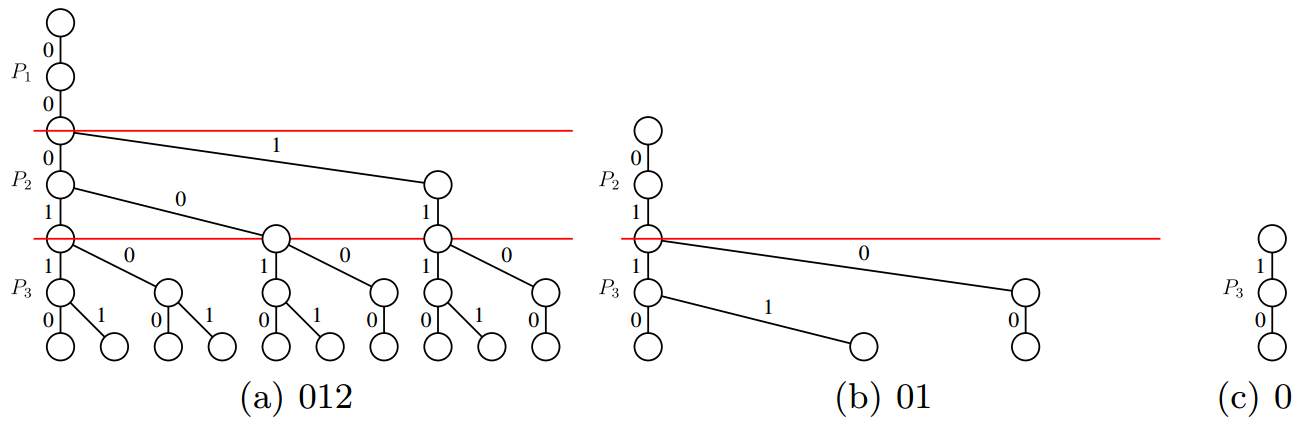
\includegraphics[width=0.92\textwidth]{images/trie.png}

\caption[Search trees from pattern `000110' using a binary alphabet, bringing rise to filters 012, 01 and 0 and three blocks, $P_1, P_2, P_3$]{Search trees\protect{}\footnotemark{} from pattern `000110' using a binary alphabet, bringing rise to filters 012, 01 and 0 and three blocks, $P_1, P_2, P_3$ (a) 3-block query for `100110' using filter 012. (b) 2-block query for `0110' using filter 01. (c) 1-block query for `10' using filter 0.}
\label{fig:filter_search}

\end{figure}
\FloatBarrier
\footnotetext{This Figure is taken from Kucherov \cite{kuch2014}}

% This algorithm relies on lemma \ref{lemma2} much like the substring filter algorithm relied on \ref{lemma1}; The lemma guarantees that for an arbitrary solution's match in the text $Y$, for at least one query, the branching behavior described above should be \gls{sufficiently lenient} such that it can match symbols all the way to the end of the pattern without eliminating the \gls{match location} for $Y$ from the set. As such, upon reaching the end of the the query string, the search generates a \gls{candidate}. Unlike the previous algorithm, many branches of the search tree may find their own such candidate sets. The return result of such a query is the union of all these sets.
 
The correctness of the suffix filter algorithm relies on the \textit{consequent} of lemma \ref{lemma2}. An arbitrary search query is \textit{not} guaranteed to find an arbitrary string $Y$ in the text; However, the lemma guarantees that \textit{at least one} search query for a suffix block sequence will have enough errors to spare throughout the search all the way to the end of the matching substring with $Y$ in the text, where it would generate a candidate to cover the \gls{solution} containing $Y$. As with the substring P2 algorithm, not all candidates necessarily correspond to solutions, as the search is `blind' to the symbols in blocks that prefix the first block of the query.
 
Observe that the suffix filters conduct a more \textit{thorough} search process, with blind sections for matches only on \textit{one} side, instead of on \textit{both} sides as was the case with substring filters. The suffix filter algorithm generally produces far fewer candidates, as it searches further to potentially thin out the match location sets than the substring filter algorithm does before generating candidates. Also observe that the \gls{search step} of the suffix filter algorithm takes longer, as it needs to spend more time searching more symbols \textit{with} recursive branching. In this sense, the suffix filter algorithm makes more extensive use of the text index than the substring filter algorithm.